%
% Modification History
%
% 2003-February-6  Jason Rohrer
% Created.
%


\documentclass{acm_proc_article-sp}
\usepackage{graphs}

\newcommand{\tw}{token\_word}

\begin{document}

\title{\tw:  Building a Xanalogical System in Ten Days}

\numberofauthors{1}

\author{
\alignauthor Jason Rohrer\\
    \affaddr{University of California, Santa Cruz}\\
    \affaddr{Dept. of Computer Science}\\
    \affaddr{Santa Cruz, CA 95064}\\
    \email{rohrer@cse.ucsc.edu}
}

\date{February 6, 2003}


\maketitle

\begin{abstract}
We describe \tw, a web-based xanalogical hypertext system.  Our system supports almost every feature associated with Xanadu, an architecture that has been actively discussed for nearly forty years.
Features include deep quotation, unbreakable references, two-way reference chasing, and frictionless micropayments that are backed by real-world currency.
To our knowledge, \tw \ is the first xanalogical system implementation to included all of these features.  Furthermore, \tw \ is the first xanalogical system of any kind to be accessible by a web browser with no additional software.

Though previous attempts at xanalogical implementations took many years and ultimately were never completed, \tw \ was implented from scratch in ten days by one person.  
We attribute this success to the maturity of modern technology and design techniques.  
In particular, choosing Perl as the implementation language allowed the rather complex xanalogical text processing operations to be expressed in elegant ways.
A live \tw \ system is running at:
\begin{center}
http://hypertext.sf.net/token\_word
\end{center}
\end{abstract}

\category{H.5.4}{Information Interfaces and Applications}{Hypertext/Hypermedia}[Architectures]
\category{K.4}{Computers and Society}{Electronic Commerce}[Payment Schemes]


\terms{Design, Human Factors}

\keywords{Micropayments, quotation, transclusion, Xanadu}

\section{Introduction}
Xanadu has been floating in the collective mind of the hypertext research community for nearly forty years.
Xanadu is a dream and an ideal.  
We know it would be great (or at least interesting) if a xanalogical system existed, but we are also resigned to the notion that such a system will probably never exist.
Is Xanadu impossible?

That question by itself, the impossibility question, is extraordinarily intriguing.  We {\it know} that Xanadu is not impossible.  
The design, on paper \cite{NelsonLiteraryMachines}, is clear enough:  we just need to build it.  
The problem might be that no one tried to build it.  
But many people did try to build Xanadu over the years.  
The problem might be that the people trying to build it did not have sufficient resources.  But people with extraordinary resources did try to build it.  
Will anyone argue that Autodesk did not have extraordinary software development resources in the late 1980s?  
Furthermore, Autodesk {\it believed} in Xanadu.  
The following quote from a 1988 Autodesk press release is most telling:

\begin{quote}
In 1964, Xanadu was a dream in a single mind.  In 1980, it was the
shared goal of a small group of brilliant technologists.  By 1989, it
will be a product.  And by 1995 it will begin to change the world.
Much work remains to be done to realise the potential of Xanadu---it
will take the Xanadu development team 18 months to field the first
Xanadu system. \cite{AutodeskPress} 
\end{quote}

In the same press release, Autodesk claimed 1987 sales figures topping \$79 million.  
Indeed, Autodesk had extraordinary resources for its time.  
In 1992, after four years of development and \$5 million spent \cite{AutodeskCost},  Autodesk ceased development of Xanadu \cite{AutodeskPressDrop}.  
Ironically, this decision was made just when the world was ripe for the first global hypertext system \cite{BernersLee92}.

We are scared of Xanadu.  
We hear its siren song and are tempted, but we know that many have tried and many have failed.  
The most frustrating factor is that none of us really know how useful Xanadu would be, even if it {\it did} exist.  
We can look at architecture diagrams and photgraphs of cardboard mock-ups \cite{Nelson1999}, but these do not give us a true sense of what it would be like to use a xanalogical system.  
Few of us have ever played with a xanalogical user interface prototype, even fewer have paid or received a true micropayment (xanalogical or otherwise), and almost none have transcluded the work of another or had our work transcluded.

What is using a xanalogical system really like?
Is it as useful as it sounds?
What made implementing Xanadu so difficult for so many people?  
This paper attempts to answer these question by describing the first fully-realized xanalogical implementation.

Given this historical perspective, the contributions of this paper are threefold.
First, this paper analyzes the process that lead from a paper design to real world xanalogical software.
Second, this paper shows that modern technology and techniques are of utmost importance for making this implementation process {\it possible}, let alone quick.
Third, this paper describes a full xanalogical system implementation from the perspective of an end-user.
The novelty of this paper hinges on the implmentation, which has a modern flavor, though the underlying ideas are quite old.
We have acheived a novel success, where past attempts have failed, and we feel that the lessons learned from this process are valuable.




\section{The Xanadu Model}

As mentioned in the above quote, Xanadu's underlying ideas were first incubated by Nelson in the 1960s \cite{Nelson1965}.  
These ideas evolved somewhat over the next forty years, receiving one of their most verbose presentations in Nelson's book {\it Literary Machines}, which was first published in 1981 \cite{NelsonLiteraryMachines}.  
Nelson's more recent paper on the xanalogical model is up to date in terms of modern technological trends, but the core ideas have not changed \cite{Nelson1999}.  
The high-level description and interpretation of Xanadu given here is based on information culled from {\it Literary Machines}, Nelson's recent lectures, and personal conversations with Nelson.

The chief goal of Xanadu, distilled into a single phrase, is {\it frictionless content reuse}.  
This goal would be easily realized in a frictionless, copyright-free world:  authors could simply copy whatever they want and reuse it however they please.  
In our world, however, we have copyright.
Unlike other systems \cite{Clark2000}, Xanadu does not attempt to undermine copyright, but instead tries to work with it. 
All of the design choices and complications in the Xanadu model can be seen as mechanisms for making reuse frictionless in the face of copyright.
When trying to implement unrestricted reuse in a way that works with copyright, we are faced with the following issue:  {\it copyright forbids unrestricted copying}.

Xanadu's central mechanism is {\it transclusion}, a form of quotation.  
Transclusion differs from standard quotation in that it does not involve copying of any kind.  
When document $A$ transcludes a quote from document $B$, the quote is stored as a deep reference to the quoted material in $B$:  words from $B$ are not copied into $A$. 
Whenver $A$ is viewed, the words from $A$ are fetched from $A$'s owner, and the necessary words from $B$ are fetched from $B$'s owner.
Thus, even though $A$'s owner has quoted document $B$, the quoted owner still retains control over the distribution and licensing of his or her words.
%Avoiding copying led us to transclusion, and making transclusion work will lead us to the rest of the Xanadu model.

Transclusion creates a serious problem, at least in combination with how we commonly interact with electronic documents.
Electronic documents change constantly.
If $B$ changes or is deleted, $A$'s quote can break.
Xanadu's solution is to forbid document change but encourage document versioning.
Thus, as $B$ is updated, all previous versions are maintained, and $A$'s quote can point to the particular version that $A$'s owner quoted.
A particular version of $B$ is immutable, so $A$'s quote will never break.

The Xanadu model refines versioning further by describing an ever-growing, add-only, content space.  
When a document is created, its text is added to this space.
When a document transcludes from another document, it points not to the document itself, but to the transcluded words in the content space.
Thus, a document in Xanadu is a list of pointers to regions in the content space---no text is contained in the documents themselves.
Versioning with this mechanism is particularly space-efficient:  unchanged portions of a new document version can be transcluded from the content space instead of being duplicated.

Along with requiring a new model for document maintenance, transclusion pushes us toward a new model for licensing copyrighted material.
We commonly think about licensing documents only in their entirety.
For example, we may assign monetary value to a printed copy of a book, but we have difficulty imagining how much a chapter, page, or paragraph of that book is worth.
In the Xanadu model, when users read a quote from document $B$ embedded in document $A$, they may only be accessing a small portion of $B$ (for example, a single sentence from a 10,000-word document).
Thus, $B$'s owner must be prepared to license only a portion of $B$ to readers.
The Xanadu model handles this licensing issue with micropayments and per-character values for content.
Nelson is fond of using the term {\it nanobuck} ($10^{-9}$ dollars) to describe the smallest unit of payment:  documents, or portions of documents, are licensed for $N$ nanobucks per character.
For example, if $N=100$, a document containing one million characters, if licensed in its entirety, would cost \$0.10, while the first half would cost only \$0.05.

When licensing a portion of a document in the Xanadu model, users are actually licensing a region of the content space.
Each character in the content space can be permanently acquired for a one-time licensing fee.
Thus, if users purchase documents that overlap with regions they already own, they only pay for the portions that they have yet to acquire.
Each user accumulates a ``library'' of acquired text regions over time and pays for each region only once.

When a document is accessed that contains quotes from multiple authors, the micropayments are divided and routed to the original authors on a per-character basis. 
Though reading content requires payment, quoting is essentially free, since the content is not accessed during the act of quoting.
In practice, an author will need to read a document before quoting it, but this reading requires only the normal first-access payment, no matter how widely the new, quoting document is expected to be read.
In fact, the more a document is quoted and read in quoted form, the more micropayments the original author will receive.
Thus, authors benefit from the unrestricted quotation and reuse of their work:  they have no financial motivation for imposing any limits.

We can summarize the Xanadu model with the following feature list:  deep quotation by reference; static underlying content; and per-character, one-time micropayments.


\section{System Architecture}
We designed and built \tw, a full-featured xanalogical system, from scratch in only ten days.
To acheive this kind of rapid development, we relied heavily on modern technology and design techniques.
We do not view past Xanadu failures with disdain.
Those early attempts were simply ahead of their time:  the technology of the day was not ready for Xanadu.
The central technologies that made \tw \  development possible were the web, CGI, Perl, and PayPal \cite{paypal}.

Our system, though full-featured, was not designed to be ``the'' scalable xanalogical system that will carry us all into the future.
Instead, we focused on building a usable implemenation of xanalogical features for the purpose of experimentation.
Though scalability was not a design goal, \tw \ was built on top of technolgies that have scaled well for other web-based projects \cite{Everything2, WikiWikiWeb, Wikipedia}.
We claim that \tw \  could be scaled into a globally accessible system, albeit with minor code modifications and a sufficient hardware investment. 

\subsection{User Perspective}
In describing the \tw \ user experience, we are faced with the very issue that motivated \tw \ development in the first place:  descriptions in words and pictures do not give us a true sense of what it is like to {\it use} a system.
Since this paper's focus is on a real-world implementation and not just a paper description, we encourage readers to visit {\tt http://hypertext.sf.net/token\_word} to try our system for themselves. 

From the end-user's perspective, \tw \ has many sal\-ient features.
Users access \tw \ with a web browser, and they must create accounts and log in to use the system.  
The central elements of the system are documents, which can contain quotes of other documents.
Quote markers can be hidden or displayed, and quotes can be followed to see the context from which they were taken.
Each document also features a list of documents that quote it, so references can be chased in both directions.
The \tw \  document display interface can be seen in Figure \ref{fig:mainScreen}.

% opera window size for figures:
% 737 x 528
\begin{figure}[t]
\centering
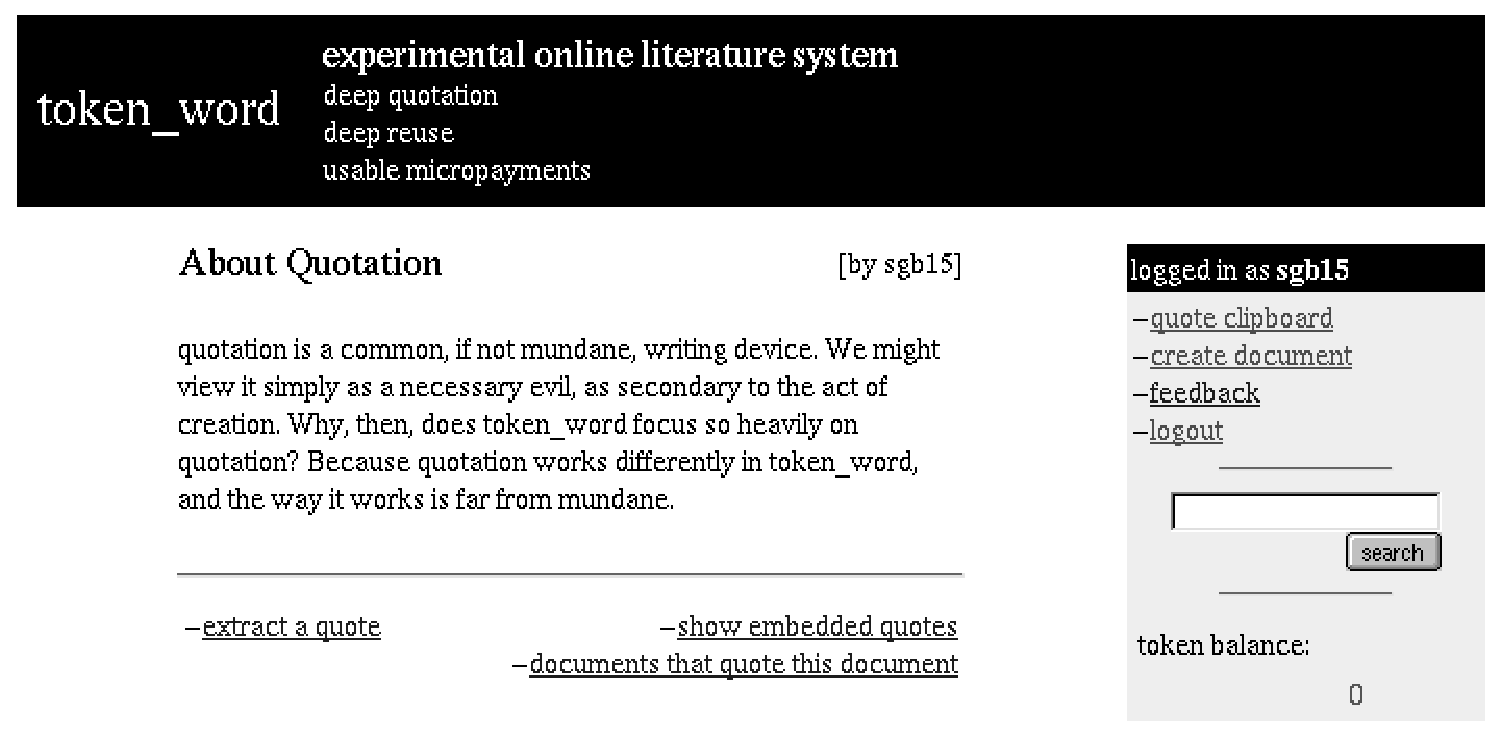
\epsfig{file=images/mainScreen.eps, width=20pc}
\caption{The document display interface.}
\label{fig:mainScreen}
\end{figure}  

Quotes can be extracted from documents and saved to a user's quote clipboard for later reference or use.
Figure \ref{fig:extractQuote} shows the interface for quote extraction. 
Quotes on a clipboard can be followed to see quote context.
The clipboard interface is shown in Figure \ref{fig:quoteClipboard}.
When creating a new document, a user can enter new text along with references to quotes from his or her quote clipboard, as seen in Figure \ref{fig:docCreate}.
A preview mode shows the new document with all quote references expanded, as seen in Figure \ref{fig:docPreview}.

\begin{figure}[t]
\centering
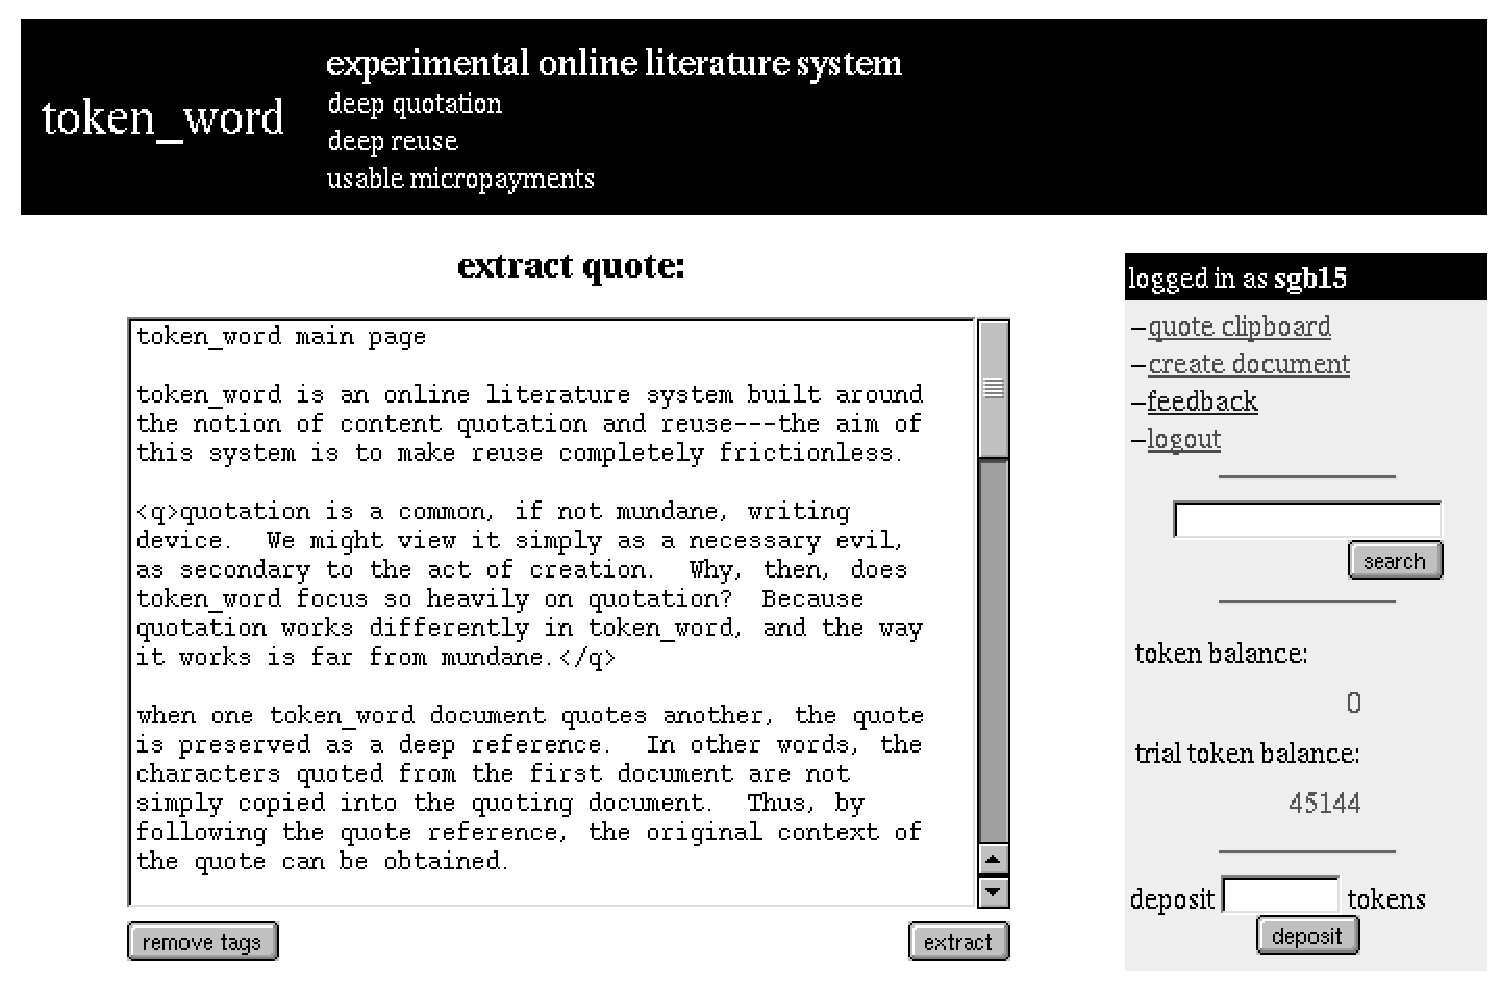
\epsfig{file=images/extractQuote.eps, width=20pc}
\caption{The interface for extracting a quote.  The region surrounded by $<$q$>$ $<$$/$q$>$ tags is selected for extraction.}
\label{fig:extractQuote}
\end{figure}

\begin{figure}[t]
\centering
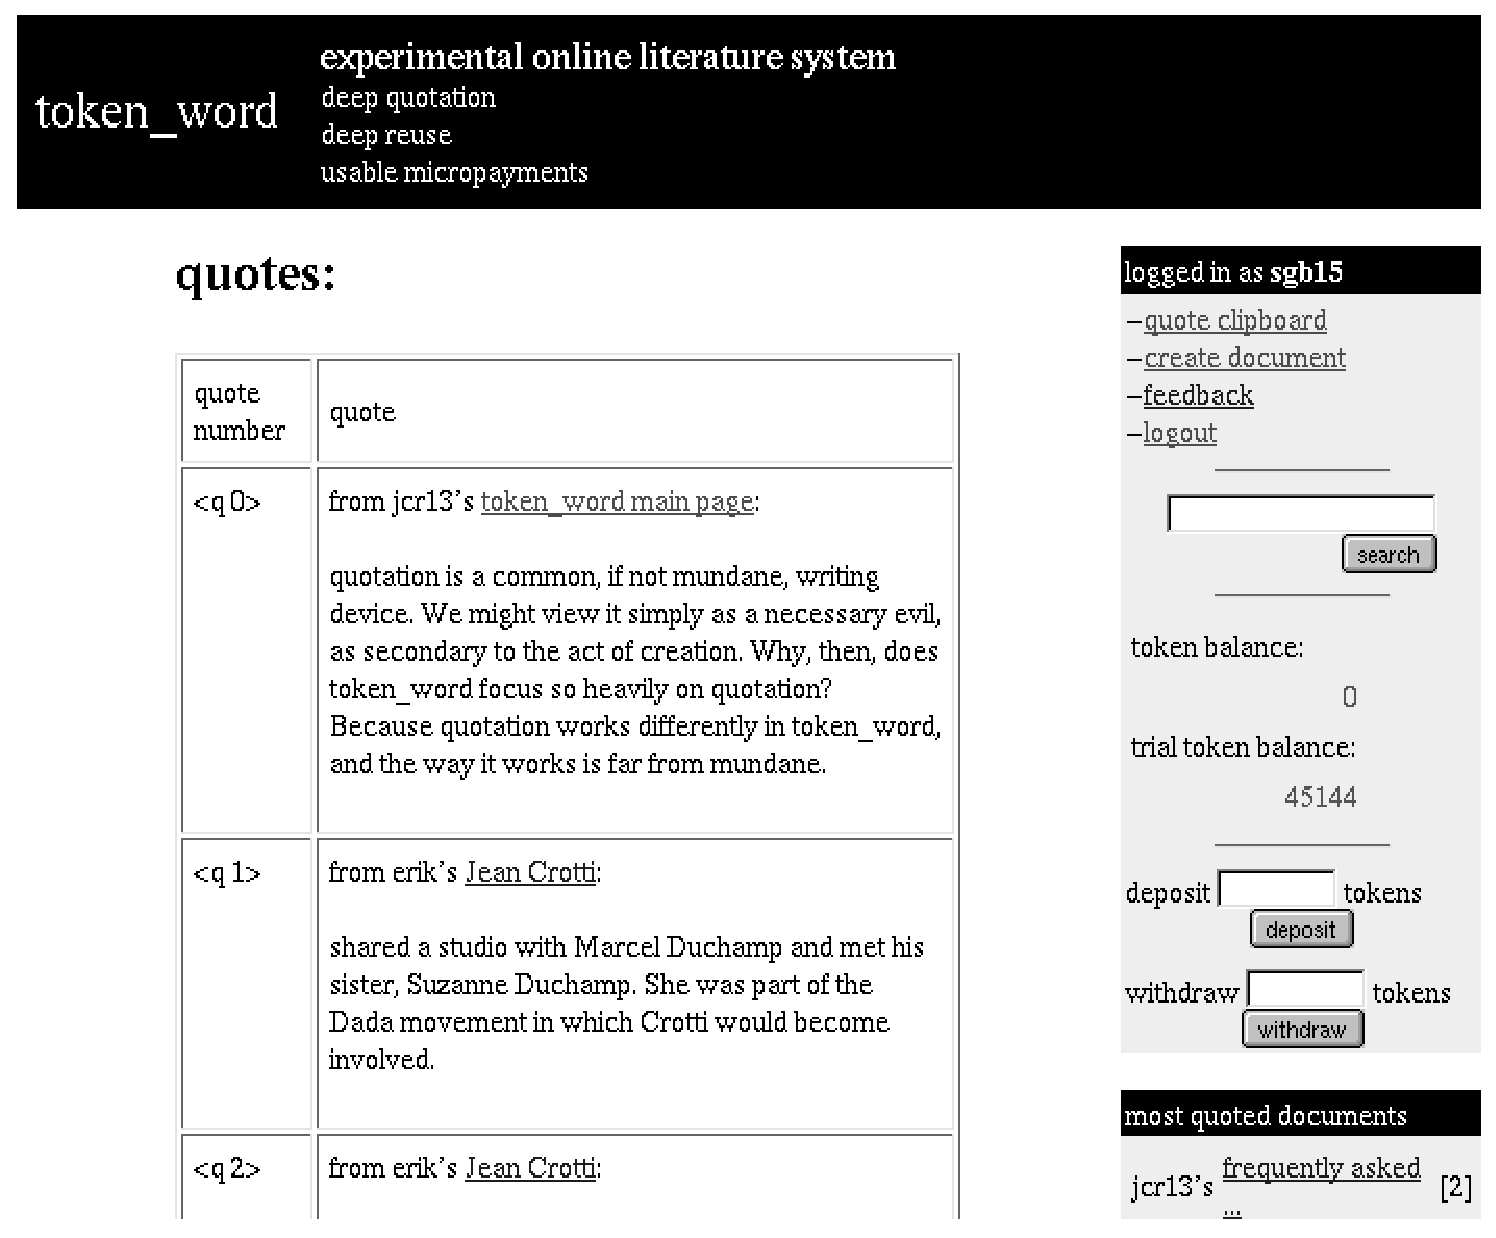
\epsfig{file=images/quoteClipboard.eps, width=20pc}
\caption{The quote clipboard interface.}
\label{fig:quoteClipboard}
\end{figure}


Each user has a token balance, where one token is worth one character.
The current exchange rate is 1,000,000 tokens for \$1, and Paypal is integrated for token deposits and withdrawls.
When a reader views a document that contains as of yet unviewed text regions, tokens are transfered from the reader to the original authors of the regions.
Users only pay for each piece of text once---repeat viewings of the same text, in any context, are free.
\begin{figure}[t]
\centering
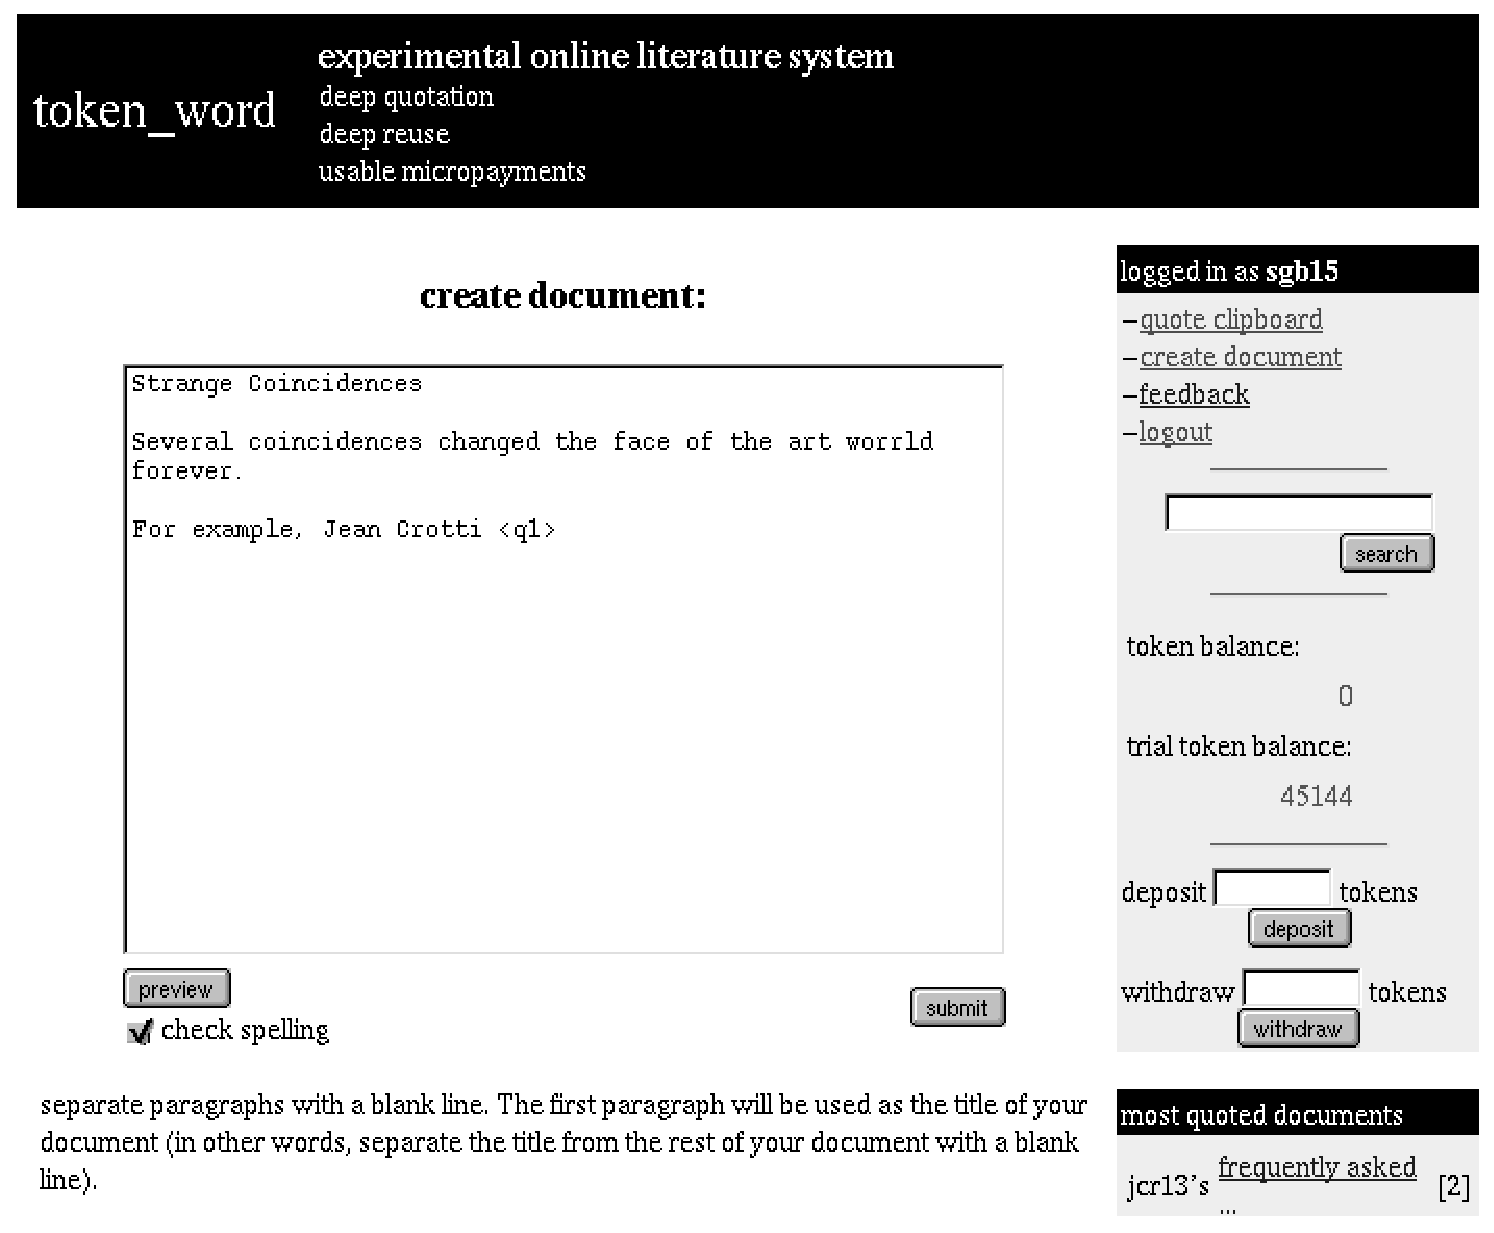
\epsfig{file=images/docCreate.eps, width=20pc}
\caption{The document creation interface. Quote 1 from the clipboard is inserted with the $<$q1$>$ tag.}
\label{fig:docCreate}
\end{figure}

\begin{figure}[t]
\centering
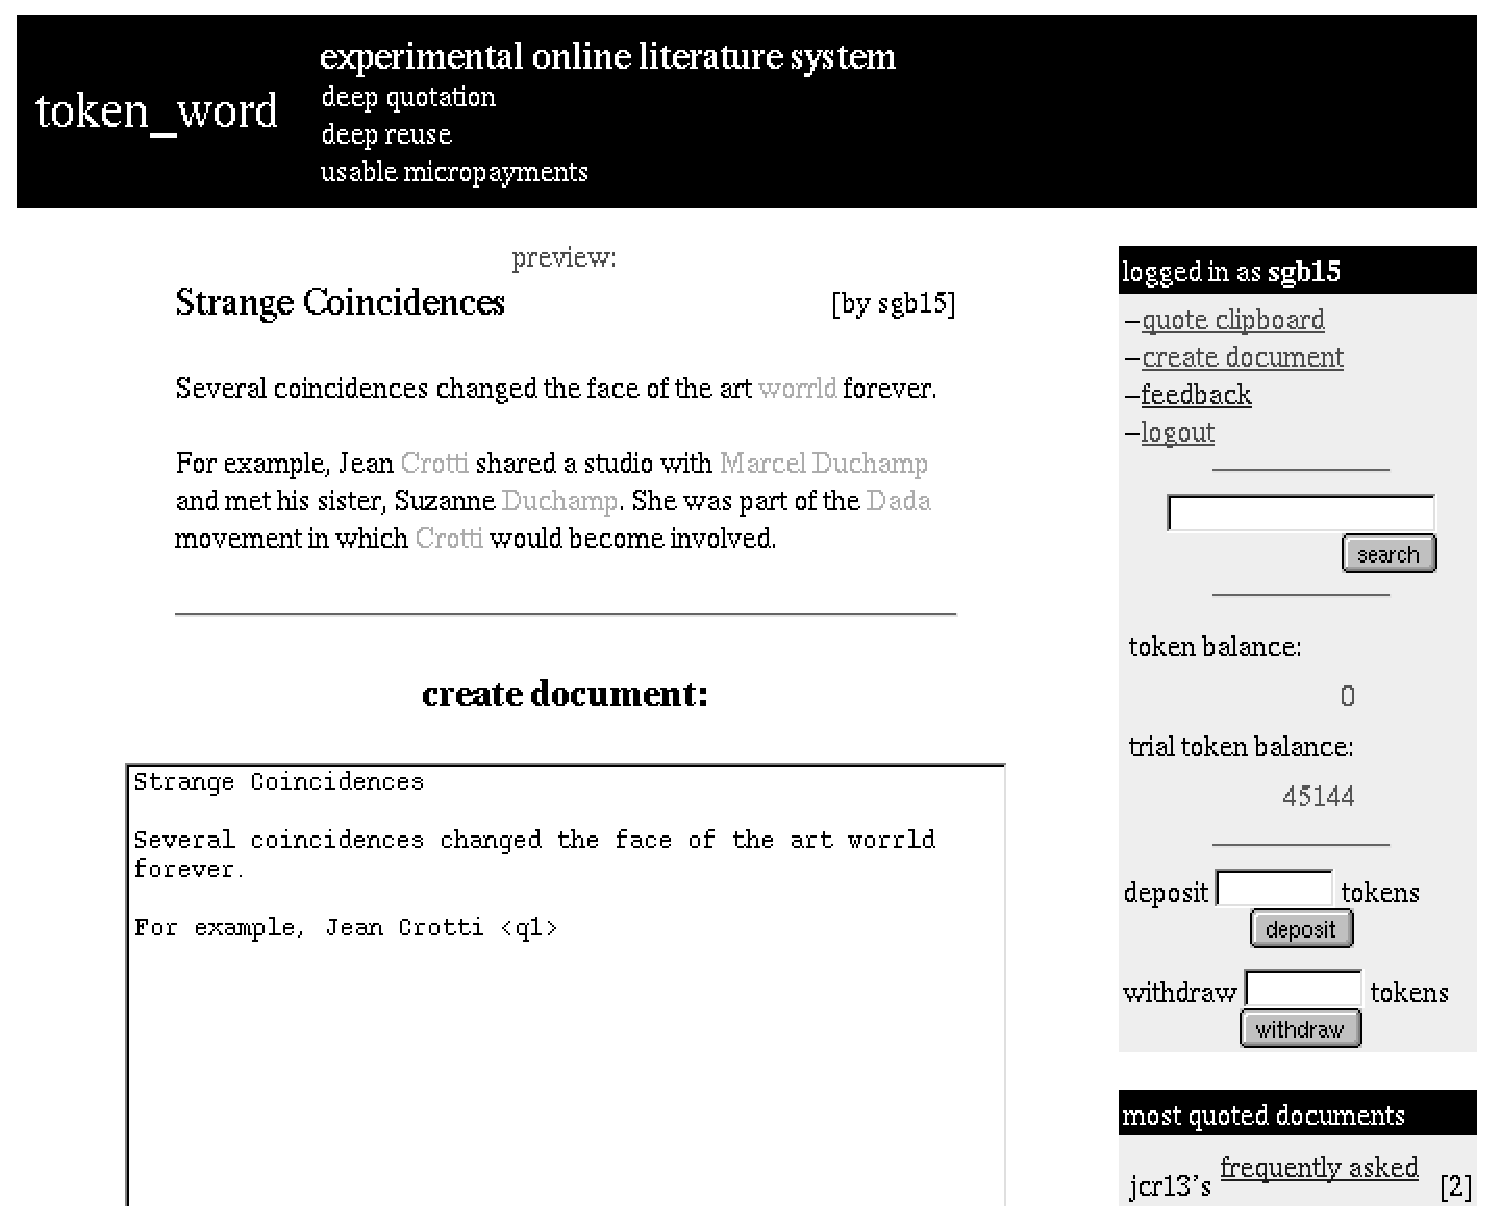
\epsfig{file=images/docPreview.eps, width=20pc}
\caption{The document preview interface.  Quotes are expanded, and possible spelling mistakes are highlighed.}
\label{fig:docPreview}
\end{figure}

Full text searches are supported across the entire document database, and search terms are highlighted when result documents are displayed.
Search results (and other lists in \tw) are sorted with most-quoted documents first, since frequently quoted documents are likely to contain the best information. 

\tw \ provides no explicit linking mechanism.
However, since quote context can be obtained easily, brief quotes can be used as links between documents.
For an example of quotes used to link, see Figure \ref{fig:quotesAsLinks}.

\begin{figure}[t]
\centering
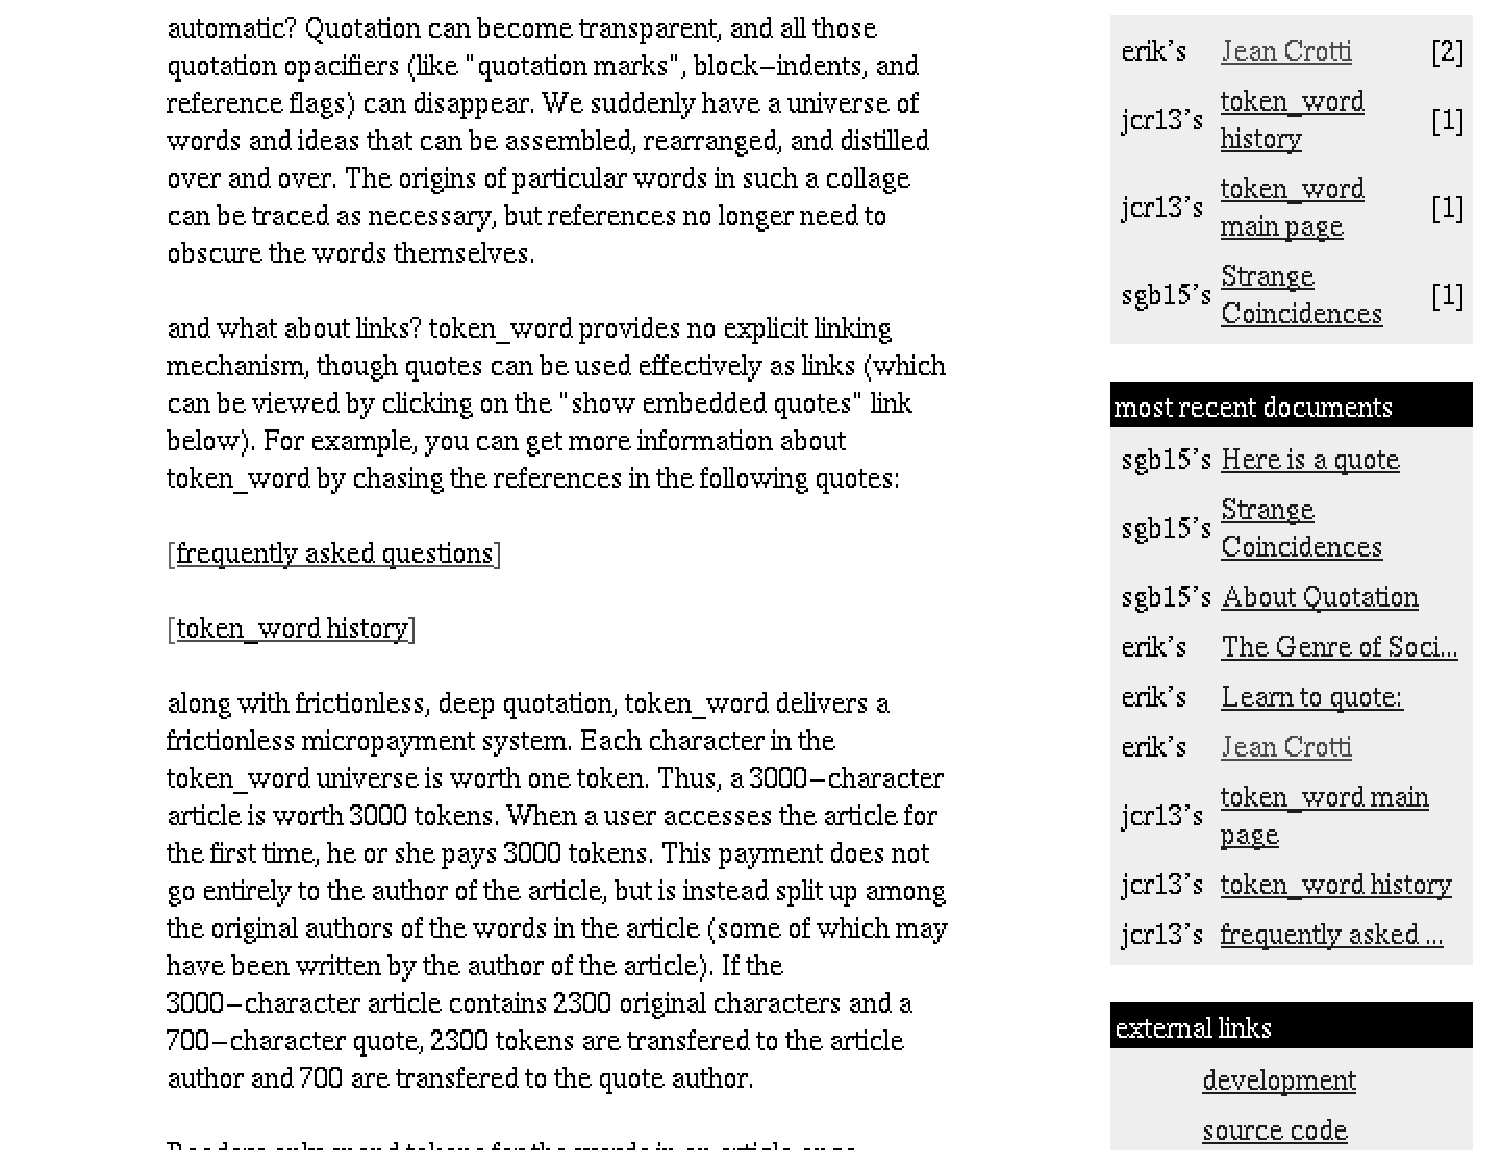
\epsfig{file=images/quotesAsLinks.eps, width=20pc}
\caption{Brief portions of documents can be quoted to form links.}
\label{fig:quotesAsLinks}
\end{figure}

\subsection{Implementation Details}

\subsubsection{Data Model}
Keeping with the Xanadu model, \tw \ separates documents from the text they contain.
There are two types of data objects in \tw:  documents and chunks.
A chunk contains a raw block of contiguous text, while a document is a list of reference to text chunks.
Some of the referenced chunks in a document may have been created at the same time as the document (for new text in the document), while others may be part of quotes taken from other documents.

Each reference in a document contains a pointer to text chunk region and an optional pointer to a document context region.
The document context pointer tracks which document the material was quoted from and is used for quote reference chasing.
If a document refers to a new text chunk that has not appeared in any previous documents, the document context pointer is omitted:  such chunks are not part of quotes and have no references that can be chased.
With this two-pointer model, we can distinguish ``original'' material in a document from quoted material and support recursive reference chasing.
When following a quote reference, a chain of referneces may need to be chased before the original context of the text is found. 

For example, suppose that document $A$ quotes a block of text from $B$, and that block contains a quote original material, residing in chunk $k$, from document $C$.  
$A$'s reference will contain both a pointer to the text chunk $k$ and to the document context $B$.  
$B$'s reference will point to both chunk $k$ and document $C$.  
At the end of this reference chain, $C$'s reference will point only to $k$.
Figure \ref{fig:referenceChain} shows a diagram of this reference chain.



\begin{figure*}[t]
\begin{center}

\begin{graph}(8,4)(-4,-1.65)
\graphnodesize{0.6}
\graphnodecolour{1}
\opaquetextfalse

\rectnode{A}[1.5,2](-6,0)[\fillednodesfalse]     
\nodetext{A}(0,1.25){Document $A$}
\rectnode{AQuote}[1.5,0.75](-6,.25)[\graphnodecolour{0.5}]  
\rectnode{kInA}[1.5,0.5](-6,.25)[\graphnodecolour{0.85}]
\roundnode{kInAStartAnchor}(-5.25,.5)[\graphnodecolour{0}\graphnodesize{0}]
\roundnode{kInAEndAnchor}(-5.25,0)[\graphnodecolour{0}\graphnodesize{0}]

\roundnode{QuoteInAStartAnchor}(-5.25,.625)[\graphnodecolour{0}\graphnodesize{0}]
\roundnode{QuoteInAEndAnchor}(-5.25,-.125)[\graphnodecolour{0}\graphnodesize{0}]


\rectnode{B}[1.5,2](-2,0)[\fillednodesfalse]
\nodetext{B}(0,-1.25){Document $B$}
\roundnode{kInBAnchor}(-1.45,-.5)[\graphnodecolour{0}\graphnodesize{0.1}]
\rectnode{AQuoteInB}[1.5,0.75](-2,-.5)[\graphnodecolour{0.5}]
\rectnode{BQuote}[1.5,0.5](-2,-.5)[\graphnodecolour{0.85}]

\roundnode{AQuoteInBStartAnchor}(-2.75,-.125)[\graphnodecolour{0}\graphnodesize{0}]
\roundnode{AQuoteInBEndAnchor}(-2.75,-.875)[\graphnodecolour{0}\graphnodesize{0}]

\roundnode{QuoteInBStartAnchor}(-1.25,-.25)[\graphnodecolour{0}\graphnodesize{0}]
\roundnode{QuoteInBEndAnchor}(-1.25,-.75)[\graphnodecolour{0}\graphnodesize{0}]


\rectnode{C}[1.5,2](2,0)[\fillednodesfalse]      
\nodetext{C}(-.75,1.25){Document $C$}
\rectnode{kInC}[1.5,1](2,0)[\graphnodecolour{.85}]
\rectnode{BQuoteInC}[1.5,0.5](2,.125)[\graphnodecolour{0.85}]

\roundnode{BQuoteInCStartAnchor}(1.25,.375)[\graphnodecolour{0}\graphnodesize{0}]
\roundnode{BQuoteInCEndAnchor}(1.25,-.125)[\graphnodecolour{0}\graphnodesize{0}]

\roundnode{kInCStartAnchor}(2.75,.5)[\graphnodecolour{0}\graphnodesize{0}]
\roundnode{kInCEndAnchor}(2.75,-.5)[\graphnodecolour{0}\graphnodesize{0}]



\rectnode{k}[1.5,1](6,0)[\graphnodecolour{.85}]      
\autonodetext{k}[n]{Chunk $k$}
\rectnode{QuoteInK}[1.5,0.5](6,.125)[\graphnodecolour{0.85}]
\roundnode{QuoteInKStartAnchor}(5.25,.375)[\graphnodesize{0}\graphnodecolour{0}]
\roundnode{QuoteInKEndAnchor}(5.25,-.125)[\graphnodesize{0}\graphnodecolour{0}]

\roundnode{kStartAnchor}(5.25,.5)[\graphnodecolour{0}\graphnodesize{0}]
\roundnode{kEndAnchor}(5.25,-.5)[\graphnodecolour{0}\graphnodesize{0}]




\diredge{QuoteInAStartAnchor}{AQuoteInBStartAnchor}[\graphlinedash{4 4}\grapharrowtype{2}]
\diredge{QuoteInAEndAnchor}{AQuoteInBEndAnchor}[\graphlinedash{4 4}\grapharrowtype{2}]
\dirbow{kInAStartAnchor}{QuoteInKStartAnchor}{0.17}[\grapharrowtype{1}]
\dirbow{kInAEndAnchor}{QuoteInKEndAnchor}{0.17}[\grapharrowtype{1}]

\diredge{QuoteInBStartAnchor}{BQuoteInCStartAnchor}[\graphlinedash{4 4}\grapharrowtype{2}]
\diredge{QuoteInBEndAnchor}{BQuoteInCEndAnchor}[\graphlinedash{4 4}\grapharrowtype{2}]

\dirbow{QuoteInBStartAnchor}{QuoteInKStartAnchor}{-0.19}[\grapharrowtype{1}]
\dirbow{QuoteInBEndAnchor}{QuoteInKEndAnchor}{-0.19}[\grapharrowtype{1}]


\dirbow{kInCStartAnchor}{kStartAnchor}{.17}[\grapharrowtype{1}]
\dirbow{kInCEndAnchor}{kEndAnchor}{.17}[\grapharrowtype{1}]


\end{graph}

\caption{An example reference chain.  Dotted lines represent document region pointers, and solid arcs represent chunk region pointers.  Light gray regions represent text from chunk $k$.  Dark gray regions in $A$ and $B$ represent portions of $A$'s quote from $B$ that do not come from chunk $k$ (other chunks are omitted from this diagram for clarity).}
\label{fig:referenceChain}

\end{center}

\end{figure*}





Quote clipboards are modeled in the following way.
Each quote on the clipboard points to a contiguous document region.
Since a  document region can be comprised of regions from multiple chunks, we might want to model each quote as a list of references, just like we model a document.
However, we simplify the clipboard by modeling each quote as a single document region pointer with no chunk region pointers.
To insert a clipboard quote into a new document, we can resolve the chunk region references for the quote and set the document region for each of these references to the document from which the quote was extracted.
This model allows us both to track the extraction context of the quote and to store the quote clipboard efficiently.
Figure \ref{fig:quoteClipboardModel} shows a diagram of a quote clipboard modeled in this way.
The alternative list model mentioned above could not be easily used to track quote extraction context, and the clipboard representation would be much larger.


\begin{figure}[b]
\begin{center}

\begin{graph}(6.5,2.5)(-3.25,-1.25)
\graphnodesize{0.6}
\graphnodecolour{1}
\opaquetextfalse


\rectnode{q0}[1.0,0.5](0,0)
\nodetext{q0}{$q0$}
\autonodetext{q0}[n]{Clipboard}
\roundnode{q0Anchor}(.5,0)[\graphnodecolour{0}\graphnodesize{0}]
\rectnode{q1}[1.0,0.5](0,-.5)
\nodetext{q1}{$q1$}
\roundnode{q1Anchor}(-.5,-.5)[\graphnodecolour{0}\graphnodesize{0}]


\rectnode{A}[1.5,2](2.5,0)     
\autonodetext{A}[n]{Document $A$}
\rectnode{AQuote}[1.5,0.75](2.5,.25)  
\roundnode{QuoteInAStartAnchor}(1.75,.625)[\graphnodecolour{0}\graphnodesize{0}]
\roundnode{QuoteInAEndAnchor}(1.75,-.125)[\graphnodecolour{0}\graphnodesize{0}]


\rectnode{B}[1.5,2](-2.5,0)     
\autonodetext{B}[n]{Document $B$}
\rectnode{BQuote}[1.5,0.5](-2.5,-.25)  
\roundnode{QuoteInBStartAnchor}(-1.75,0)[\graphnodecolour{0}\graphnodesize{0}]
\roundnode{QuoteInBEndAnchor}(-1.75,-.5)[\graphnodecolour{0}\graphnodesize{0}]



\diredge{q0Anchor}{QuoteInAStartAnchor}[\graphlinedash{4 4}\grapharrowtype{2}]
\diredge{q0Anchor}{QuoteInAEndAnchor}[\graphlinedash{4 4}\grapharrowtype{2}]

\diredge{q1Anchor}{QuoteInBStartAnchor}[\graphlinedash{4 4}\grapharrowtype{2}]
\diredge{q1Anchor}{QuoteInBEndAnchor}[\graphlinedash{4 4}\grapharrowtype{2}]

\end{graph}

\caption{An example quote clipboard.  Dotted lines represent document region pointers.}
\label{fig:quoteClipboardModel}

\end{center}

\end{figure}






\subsubsection{Data Representation}
The system data is stored in a directory tree on the filesystem.
Each user has directory that stores that user's chunk files, document files, and quote clipboard files, along with a list of previously purchased chunk regions.
To support two-way reference chasing, each document has a file that tracks the documents that quote it.

References throughout the system are stored in the following form:
\begin{center}
{\tt <chunkUserID, chunkID, startOffset, length;\\ 
docUserID, docID, startOffset>} 
\end{center}
The portion of the reference befor the ``;'' describes the text chunk of the reference.  
The second portion, which is optional, describes the quote context of the reference.  
Note that {\tt chunkUserID} may differ from {\tt docUserID}, since the quote context may be part of a quote in another document.
For example, document $A$ may quote from document $B$, but the portion that $A$ quotes may be part of $B$'s quote from document $C$.
In this example, the reference included in $A$ might look like this:
\begin{center}
{\tt <userC, C, 105, 38; userB, B, 421>} 
\end{center}
Note that {\tt length} is not specified for the document context of a reference, since it would be redundant.

With this representation, a reference can be used both to fetch the required text chunk region and to display context in case of a followed quote reference.
By following context repeatedly for a nested quotation, the original author and document context of particular words can be obtained.
When a new chunk is created as part of a document, the context portion of the reference is ommited, indicating that the document is the first context in which this chunk was used.

Since documents and text chunks are static, full text searches can be implemented using an index that is updated in real time as documents are created.
Each word in the index is associated with a list of documents containing that word.
When a document is added to the system, it is appended to the end of the index list for each word that it contains.


\subsubsection{Development}
The entire \tw \  system is implemented as a single CGI script written in Perl, though the script is broken up into eight modules for organization purposes.
Perl's built-in support for regular expressions was very useful for the rather complicated text processing done by \tw.
Many of these text processing operations could be expressed in succinct and elegant ways using Perl.
For example, highlighting possible misspellings in preview mode was a minor addition that required less than fifteen lines of code.

CGI programming is well-supported in Perl, and HTML made user interface layout and user action processing easy to implement.
Perl-based CGI programming seems to be the modern method of choice for rapidly developing complex, multi-user applications.
Other systems that have used this development method successfully are discussed in Section \ref{sec:RelatedWork}.

Even though the full development cycle was short, we used an iterative process.
Features were added one at a time to the system, and the system was maintained in a usable form at all times.
For example, we started with a system that managed text chunks, then added document management, then added quotes, then added tokens transfers, {\it etc.}
Final iterations added features such as spell checking and index-based searching.
From our understanding of previous xanalogical implementation efforts, this iterative process may have been key to our success.
The Xanadu model is complex and subtle, and it is easy to get bogged down by details without ever producing a working system.
Our system started out simple and grew in complexity, feature by feature.


\subsubsection{Implementation Limitations}
The main limitation of our implementation is the use of a filesystem as a data backend.


\subsection{Xanalogical Improvements}


\subsection{Missing Features}



\section{Micropayment Issues}


\subsection{Balancing Risk}



\section{Related Work}
\label{sec:RelatedWork}

Wikis
\cite{WikiWikiWeb}
\cite{Wikipedia}

Everything2
\cite{Everything2}

Weblogs
\cite{kuro5hin}

Xanadu

\section{Conclusion}


\section{Acknowledgements}
Thanks are due to Ted Nelson and Jim Whitehead for their contributions to interesting xanalogical discussions over the past year. ``Xanadu'' is a trademark of Ted Nelson.  To prevent confusion, the generic terms ({\it e.g.}, xanalogical system) have been used wherever possible.

\bibliographystyle{abbrv}
\bibliography{paper}
\end{document}